\section{Realisering og test}
\label{sec:research}

Kretsen i figur \ref{fig:kretsdiagram} ble realisert med komponentene i tabel \ref{tab:comp}.

\begin{table}[!tbp]
    \centering
    \caption{Komponenter brukt i differensialforsterkeren.}
    \label{tab:comp}
    \begin{tabular}{lll}
    Komponent  & type          & verdi                  \\ \hline
    Q$_1$      & 2N7000        &                        \\
    Q$_2$      & 2N7000        &                        \\
    Q$_3$      & VP2106        &                        \\
    Q$_4$      & VP2106        &                        \\
    Q$_5$      & 2N7000        &                        \\
    Q$_6$      & 2N7000        &                        \\
    R$_{P}$   & Potensiometer  & \text{10k$\Omega$}     \\
    R$_{P1}$  &                & \text{20k$\Omega$}     \\
    R$_{P2}$  &                & \text{10k$\Omega$}     \\
    R$_{S}$   &                & \text{1k$\Omega$}      \\
    R$_{I1}$  &                & \text{1.2k$\Omega$}     \\
    R$_{i2}$   &               & \text{10.8k$\Omega$}
    \end{tabular}
    \end{table}

    \begin{figure}[!hbt]
        \centering
        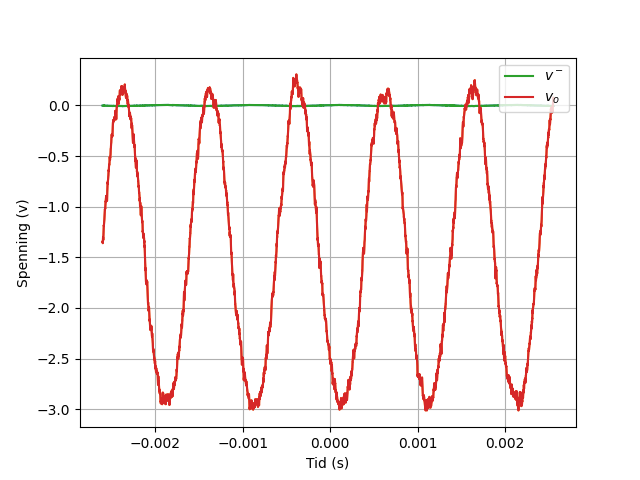
\includegraphics[scale=0.5]{./Images/03Research/åpenløkkeplain.png}
        \caption{Åpen-løkkeforsterkning med en inngangssignal på 5mV.}
        \label{fig:åpenløkke}
    \end{figure}

    Dette gav en forsterkning på $A \approx 350$ og en THD på $-27.6dB$ med en inngangssignal på 5mV og 1 KHz, det ble også observert lavere forsterkning og høyere THD ved høyere ingangssignal og når inngangssignalet gitt høyere enn 10mV så ble det observert klipping i utgangssgnalet som vist i figur \ref{fig:åpenløkke15mv}

    \begin{figure}[!hbt]
        \centering
        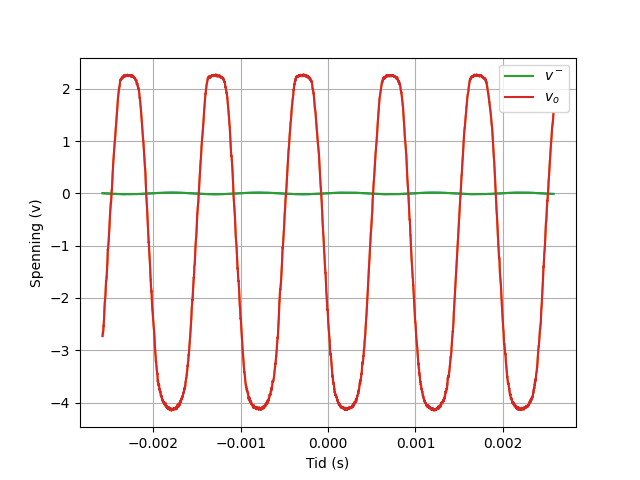
\includegraphics[width=.6\linewidth]{./Images/03Research/åpenløkkeplain15mv.png}
        \caption{Åpen-løkkeforsterkning med en inngangssignal på 15mV.}
        \label{fig:åpenløkke15mv}
    \end{figure}

Dette kan skyldes at det ikke er tilstrekkelig med spenningsforsyning $V^+$ og $V^-$ da tilsvarende klipping også forekom ved en inngangssignal på 5mV når spenningsforsyningen ble redussert.

Måling av THD og forsterkning $A$ ved sinuspåtrykk med frekvens f = 1 kHz med både 100 \text{$\Omega$} og 100 k\text{$\Omega$} er plottet inn i tabell \ref{tab:lastmotstand} utgangssignalene er vist i figur

\begin{table}[!hbt]
    \centering
    \caption{Forsterkning og THD ved ulik last motstand og type måling.}
    \label{tab:lastmotstand}
    \begin{tabular}{llll}
    Type                & $R_0$                & A      & THD[dBc]     \\ \hline
    Åpen-løkke          & 0                    & 348    & -36.7        \\
    Åpen-løkke          & 100 \text{$\Omega$}  & 91     & -7.7         \\
    Åpen-løkke          & 100 \text{$K\Omega$} & 346    & -37.0        \\
    Ikke-inverterende   & 100 \text{$\Omega$}  & 9.74   & -48.01       \\
    Ikke-inverterende   & 100 \text{$K\Omega$} & 9.83   & -59.85      
    \end{tabular}
    \end{table}

    \begin{figure}[!hbt]
        \centering
        \begin{subfigure}{.5\textwidth}
            \centering
            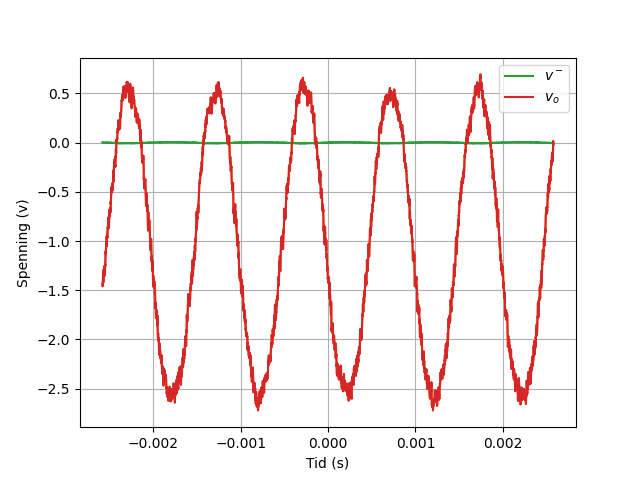
\includegraphics[width=1\linewidth]{./Images/03Research/åpenløkkeplain100kohm.png}
            \caption{Åpen-løkkeforsterkning med lastmotsand på 100 k\text{$\Omega$}}
            \label{fig:100k}
        \end{subfigure}%
        \begin{subfigure}{.5\textwidth}
            \centering
            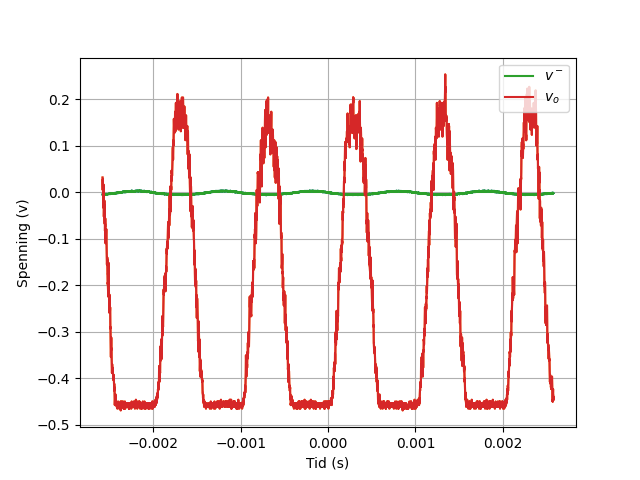
\includegraphics[width=1\linewidth]{./Images/03Research/åpenløkkeplain100ohm.png}
            \caption{Åpen-løkkeforsterkning med lastmotsand på 100 \text{$\Omega$}}
            \label{fig:100}
        \end{subfigure}
        % \caption{}
        % \label{fig:test}
    \end{figure}

    Siden spenningen blir lavere over lastmotstanden \text{$R_L$} ved lav motstand kan det tenkes at utgangsmotstanden  til systemet har noe å si da det skjer et spenningsfall før lastmotstanden i motsetning til en høy lastmotsand da tilnermet alt spenningsfallet skjer over denne.

    \begin{figure}[!hbt]
        \centering
        \begin{subfigure}{.5\textwidth}
            \centering
            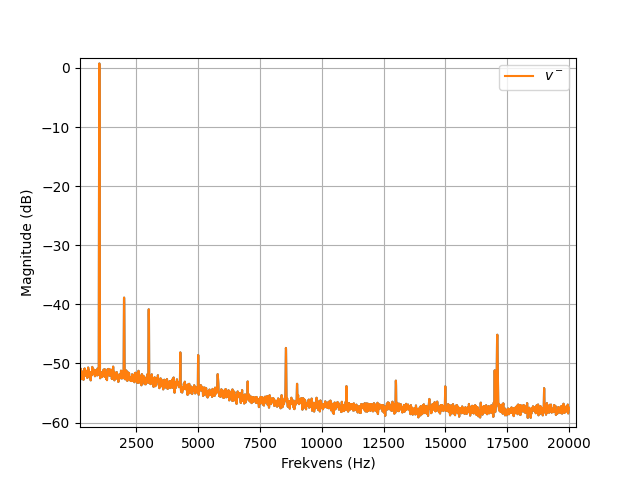
\includegraphics[width=1\linewidth]{./Images/03Research/spektrum100k.png}
            \caption{Åpen-løkkeforsterkning med lastmotsand på 100 k\text{$\Omega$}}
            \label{fig:100kspek}
        \end{subfigure}%
        \begin{subfigure}{.5\textwidth}
            \centering
            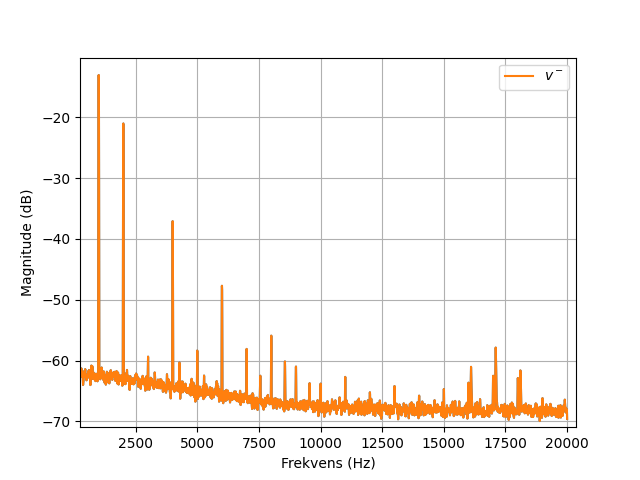
\includegraphics[width=1\linewidth]{./Images/03Research/spektrum100.png}
            \caption{Åpen-løkkeforsterkning med lastmotsand på 100 \text{$\Omega$}}
            \label{fig:100spek}
        \end{subfigure}
        \caption{Frkvensspekter for lastmotsand på 100 k\text{$\Omega$} og 100 \text{$\Omega$}}
        \label{fig:Frkvensspekter}
    \end{figure}

Det er observert at lav lastmotstand også gir mer overharmonisk støy i figur \ref{fig:Frkvensspekter}.

Ved ikke-inverterende forsterkerkobling som vist i figur \ref{fig:Ikke-inverterende} med en forsterkning $A \approx 10$ ble utgangssignalene seende som vist i figur \ref{fig:ikkeinv}, mens frekvensspekteret er plottet i figur \ref{fig:ikkeinvspek}.Da det er lavere forsterkning her så blir det brkt et høyere amplitude på inngangssignalet. Det er lite forskjell på forsterkning mellom høy og lav lastmotstand, men det forekommer mer støy på den ikke-inverterende forsterkerkoblingen med lav lastmotstand. Til tross for dette så er det generelt lavere støy og forsterkningene på 9.74 og 9.83 ganske så nerme 10 som det burde vært ifølge teorien i \cite{a2020_glossary} der det oppgis at forsterkningen skal være

\begin{equation}
    A=1+\frac{R_{I2}}{R_{I1}}
\end{equation}


\begin{figure}[!hbt]
	\centering
	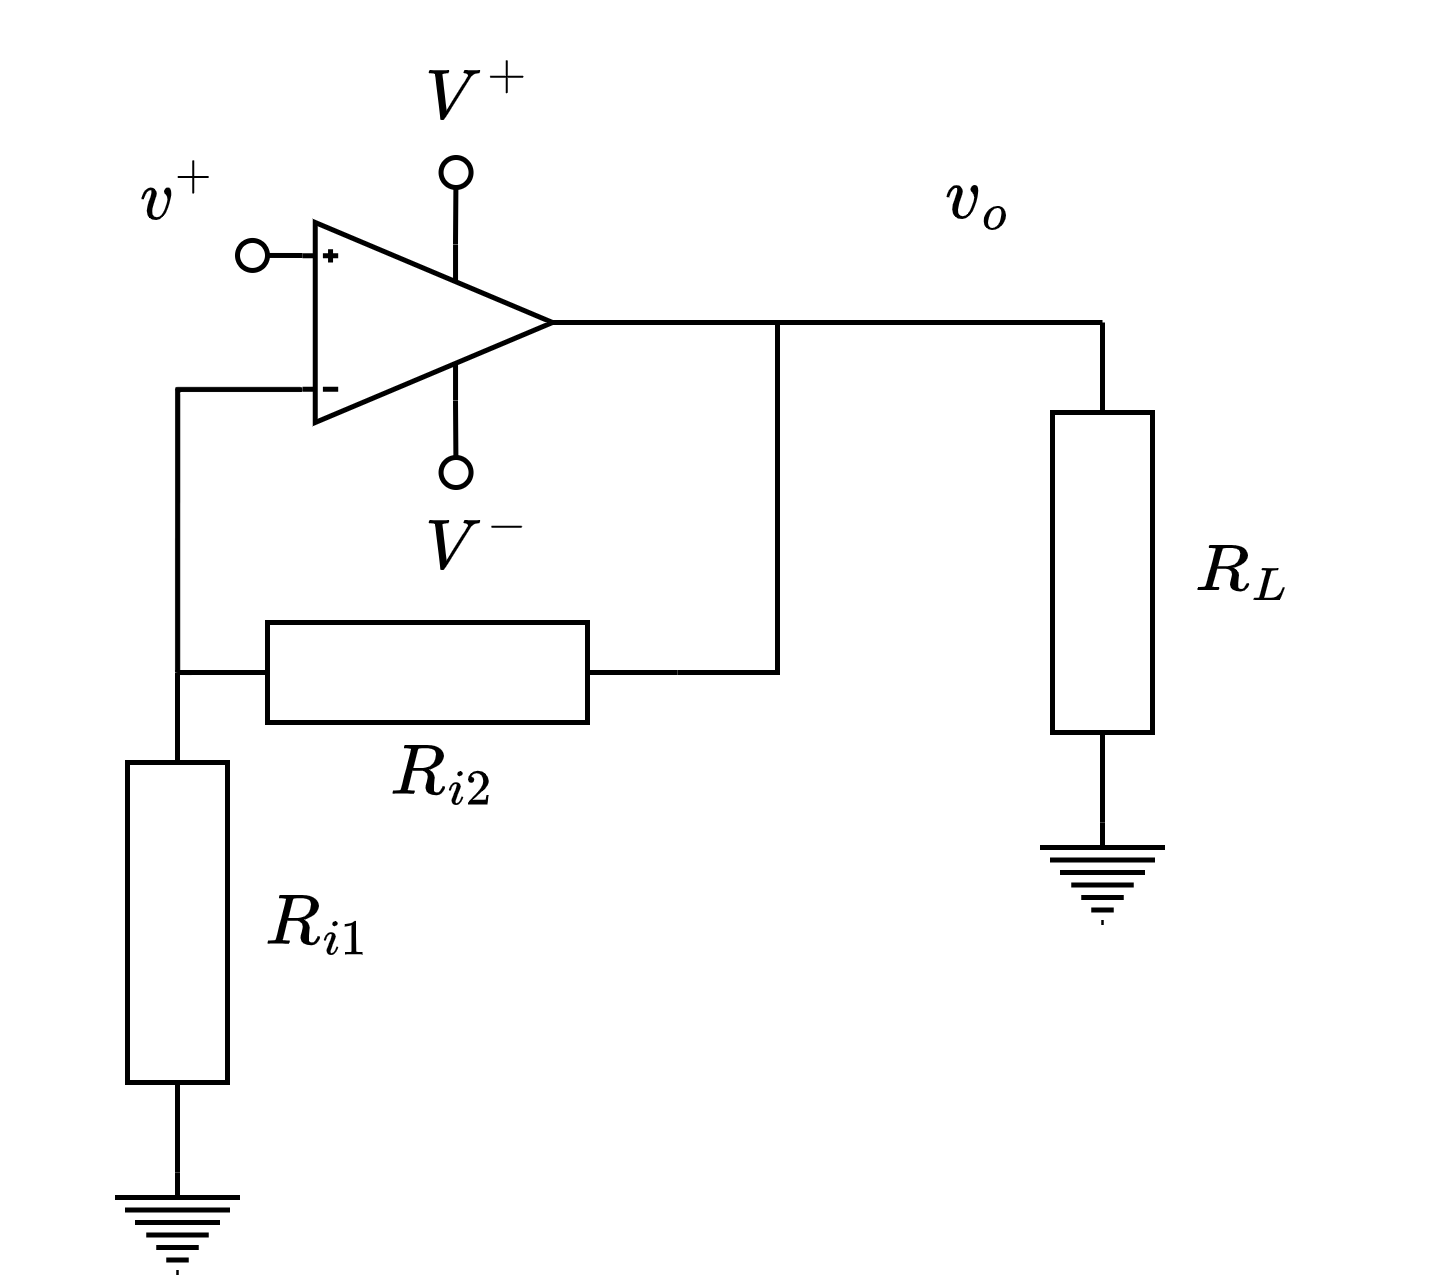
\includegraphics[scale=0.4]{./Images/03Research/ikkeinverterende.png}
	\caption{Ikke-inverterende forsterkerkobling.}
	\label{fig:Ikke-inverterende}
\end{figure}


\begin{figure}[!hbt]
    \centering
    \begin{subfigure}{.5\textwidth}
        \centering
        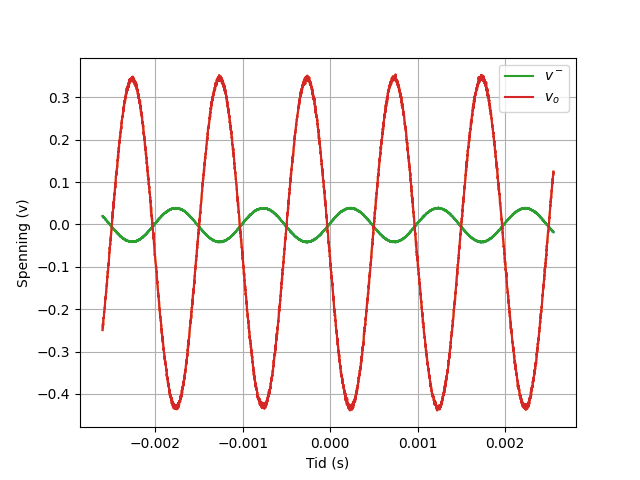
\includegraphics[width=1\linewidth]{./Images/03Research/noninverting100k.png}
        \caption{Ikke-inverterendeforsterkning med lastmotsand på 100 k\text{$\Omega$}}
        \label{fig:ikkeinv100k}
    \end{subfigure}%
    \begin{subfigure}{.5\textwidth}
        \centering
        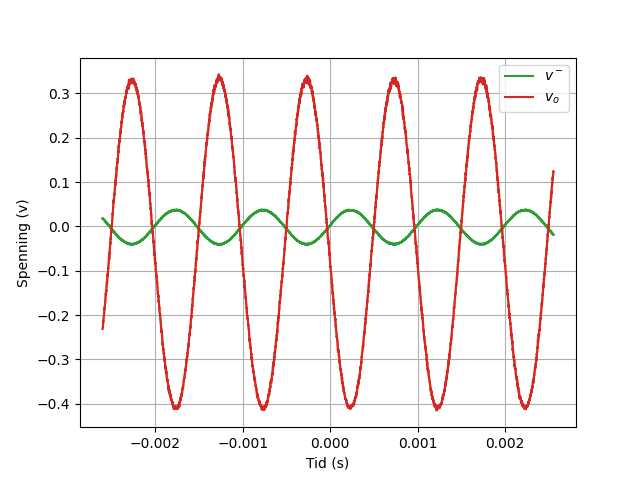
\includegraphics[width=1\linewidth]{./Images/03Research/noninverting100.png}
        \caption{Ikke-inverterendeforsterkning med lastmotsand på 100 \text{$\Omega$}}
        \label{fig:ikkeinv100}
    \end{subfigure}
    \caption{Ikke-inverterendeforsterkning med inngangssignal på 40mV.}
    \label{fig:ikkeinv}
\end{figure}

\begin{figure}[!hbt]
    \centering
    \begin{subfigure}{.5\textwidth}
        \centering
        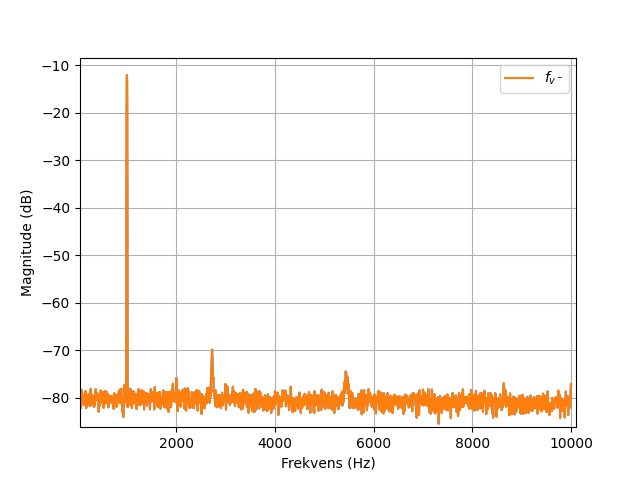
\includegraphics[width=1\linewidth]{./Images/03Research/noninvertingspektrum100k.png}
        \caption{Frekvensspekter med lastmotsand på 100 k\text{$\Omega$}}
        \label{fig:ikkeinvspek100k}
    \end{subfigure}%
    \begin{subfigure}{.5\textwidth}
        \centering
        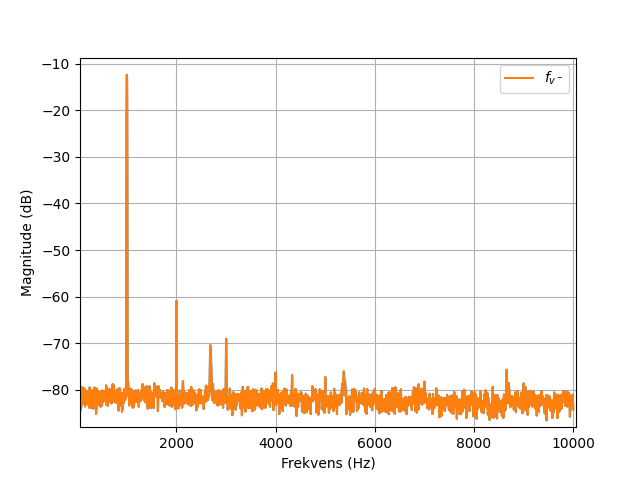
\includegraphics[width=1\linewidth]{./Images/03Research/noninvertingspektrum100.png}
        \caption{Frekvensspekter med lastmotsand på 100 \text{$\Omega$}}
        \label{fig:ikkeinvspek100}
    \end{subfigure}
    \caption{Frekvensspekter til ikke-inverterendeforsterkning med inngangssignal på 40mV.}
    \label{fig:ikkeinvspek}
\end{figure}

For å finne uv av inngangs- og utgangshastigheten blir metoden i løsningsforslaget \cite{ntnu_2022_ttt4265} brukt, der formelen for inngangsmotstanden er gitt ved

\begin{equation}
    R_i=R'\frac{v_i}{v_s}
\end{equation}

For å måle inngangsmotstanden ble det brukt en motstand på 1M$\Omega$ i figur \ref{fig:lastmot}, $v_i$ ble målt til 69mV, og $v_s$ ble målt til 42mV. Dette gir en inngangsmotstand på $R_i\approx$1.55M$\Omega$.

\begin{figure}[!hbt]
	\centering
	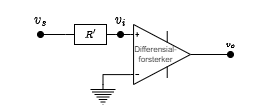
\includegraphics[scale=0.7]{./Images/03Research/lastmot.png}
	\caption{måling av inngangsmotstand.}
	\label{fig:lastmot}
\end{figure}

Ved måling av utgangsmotstanden ble en motstand brukt som vist i figur \ref{fig:outmot} der spenningen $v_o$ målt før motstanden ble satt på ble målt til 3.276V, mens $v_L$ ble målt til 1.37V. Motstanden som ble brukt var på 100$\Omega$ dermed ved bruk av formelen i LF \cite{ntnu_2022_ttt4265} så gir det en utgangsmotstand på $R_o\approx$129$\Omega$.

\begin{equation}
    R_o=R_L\frac{v_o-v_L}{v_L}
\end{equation}

brukt på kretsen i figur \ref{fig:outmot} 

\begin{figure}[!hbt]
	\centering
	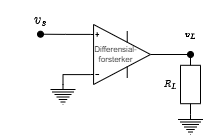
\includegraphics[scale=0.7]{./Images/03Research/outmot.png}
	\caption{måling av utgangsmotstand.}
	\label{fig:outmot}
\end{figure}